\documentclass[a4paper, 12pt]{article}
\usepackage[brazil]{babel}
\usepackage[utf8]{inputenc}
\usepackage{graphicx}
\author{Seu nome aqui}
\title{Um estudo sobre redes neurais artificiais}
\begin{document}
	\maketitle
\section{Introdução}
\subsection{Objetivos Específicos}
\begin{enumerate}
	\item Avaliar a utilização do software;
	\item Identificar os aspectos mais relevantes.
\end{enumerate}
\subsection{Redes Neurais}
A representação de um neurônio está ilustrada na Figura~\ref{fig:neuronio} e a ativação de um neurônio é descrita pela Equação~\ref{eq:ativacao}.
\begin{equation}
y_i = \sum_{i=0}^{n} w_i \times x_i
\end{equation}\label{eq:ativacao}

\begin{figure}[htb]
	\centering
	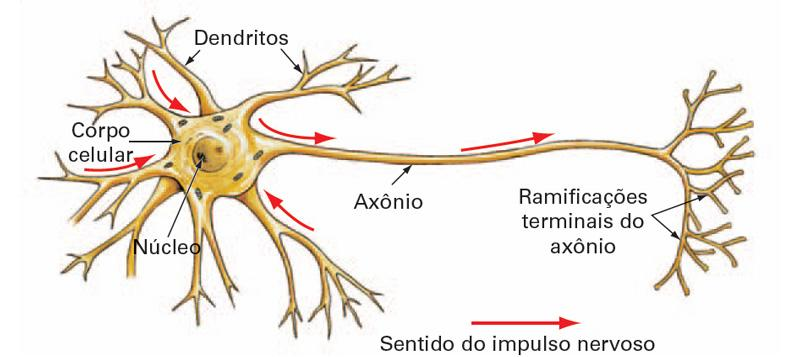
\includegraphics[scale=.5]{neuronio}
	\caption{Representação de um neurônio}\label{fig:neuronio}
\end{figure}

\end{document}
